\documentclass[letterpaper,openany,oneside,twocolumn]{book}

\newcommand{\PATH}{../../../}

\usepackage{\PATH templates/utilities/m4rz-fonts}
\usepackage{\PATH templates/utilities/m4rz-colors}

\usepackage[justified]{\PATH templates/template_dnd/dnd}

\usepackage[edition=5e24]{\PATH templates/template_character-sheet/character-sheet-stylesheet}
\usepackage{\PATH templates/template_magic-item/magic-items_commands}

\setlength\oddsidemargin{\dimexpr(\paperwidth-\textwidth)/2 - 1in\relax}
\setlength\evensidemargin{\oddsidemargin}

% CHARACTER STATS
\CharacterName{Fauna-Enhanced Automaton of Ruin}

\Class{Druid}
\MultiClassMainLevel{3}
\MultiClass{Warlock}
\Subclass{Circle of the Moon}
\Background{Compleated}
\Race{Warforged}

\Level{8}

% ABILITY SCORES
% (correct scores, no modifiers are automatically applied)
% Modifiers, Saving Throws and Skills are calculated automatically
\StrengthRolledScore{16}
\DexterityRolledScore{13}
\ConstitutionRolledScore{12}
\IntelligenceRolledScore{10}
\WisdomRolledScore{17}
\CharismaRolledScore{16}

\StrengthScoreBonus{0}
\DexterityScoreBonus{1} % Poisoner +1
\ConstitutionScoreBonus{2} % Warforged +2
\IntelligenceScoreBonus{0}
\WisdomScoreBonus{1} % ASI +1
\CharismaScoreBonus{2} % Warforged +1, ASI +1

\calculateAbilityScores{}

% PROFICIENCIES AND EXPERTIES
%% SAVING THROWS
\StrengthProficiency{}
\DexterityProficiency{}
\ConstitutionProficiency{}
\IntelligenceProficiency{P}
\WisdomProficiency{P}
\CharismaProficiency{}

%% STRENGTH SKILLS
\AthleticsProficiency{P}

%% DEXTERITY SKILLS
\AcrobaticsProficiency{}
\SleightOfHandProficiency{}
\StealthProficiency{}

%% INTELLIGENCE SKILLS
\ArcanaProficiency[\calculateModifier{\WisdomScoreValue}]{}
\HistoryProficiency{}
\InvestigationProficiency{}
\NatureProficiency[\calculateModifier{\WisdomScoreValue}]{}
\ReligionProficiency{}

%% WISDOM SKILLS
\AnimalHandlingProficiency{}
\InsightProficiency{P}
\MedicineProficiency{}
\PerceptionProficiency{P}
\SurvivalProficiency{P}

%% CHARISMA SKILLS
\DeceptionProficiency{P}
\IntimidationProficiency{P}
\PerformanceProficiency{}
\PersuasionProficiency{P}

% ABILITY MODIFIERS BONUS
\StrengthModifierBonus{0}
\DexterityModifierBonus{0}
\ConstitutionModifierBonus{0}
\IntelligenceModifierBonus{0}
\WisdomModifierBonus{0}
\CharismaModifierBonus{0}

\Inspiration{}
\PassivePerceptionModifier{0}

\ArmorClass{\intcalcAdd{12}{\intcalcAdd{1}{\calculateModifier{\DexterityScoreValue}}}}

\MaxHitPointsRolled{52} % Without Constitution Bonus, is added automatically
\CurrentHitPoints{\MaxHitPointsValue}
\TemporaryHitPoints{}
\HitDice{d8}
\MultiClassHitDice{d8}
\HitDiceSpent{0}
\MultiClassHitDiceSpent{0}

\InitiativeModifier{0}
\Speed{30}
\Size{Medium}

\LightArmor{P}
\MediumArmor{P}
\HeavyArmor{}
\Shields{P}

\WeaponsProficiency{Simple Weapons, Martial Weapons}
\ToolsProficiency{Herbalism Kit, Poisoner's Kit}

\addWeaponStatistic{Quarterstaff}{F.E.A.R}{STR}{P}{0}{1d6 b}{versatile (1d8)}
\addWeaponStatistic{Armblade}{F.E.A.R}{STR}{P}{+1}{1d8 s}{heavy}
\addWeaponStatistic{Unarmed Strike}{F.E.A.R}{STR}{P}{+1}{\intcalcAdd{2}{\calculateModifier{\StrengthScoreValue}} b}{}

\addSpellStatistic{Eldritch Blast}{ATK}{\calculateModifier{\CharismaScoreValue}}{1d10 F}{2 Beams}
\addSpellStatistic{Frostbite}{DC}{\calculateModifier{\WisdomScoreValue}}{2d6 C}{Target has disadvantage on next weapon attack}
\addSpellStatistic{Infestation}{DC}{\calculateModifier{\WisdomScoreValue}}{2d6 P}{Target must run away}
\addSpellStatistic{Primal Savagery}{ATK}{\calculateModifier{\WisdomScoreValue}}{2d10 A}{}
\addSpellStatistic{Starry Wisp}{ATK}{\calculateModifier{\CharismaScoreValue}}{2d8 R}{Target glows and cannot be invisible}
\addSpellStatistic{Toll the Dead}{DC}{\calculateModifier{\CharismaScoreValue}}{2d8 N}{or 2d12 N if target is missing health}

\AddClassFeature{B}{\textbf{Wild Shape}\\2 Uses}
\AddClassFeature{E}{\textbf{Circle Forms}\\AC \intcalcAdd{13}{\intcalcAdd{1}{\calculateModifier{\WisdomScoreValue}}}, max CR 1, 9 temp HP}
\AddClassFeature{L}{\textbf{Form of the Dread}\\\intcalcAdd{0}{\ProficiencyValue} Uses}
\AddClassFeature{E}{\textbf{Eldritch Invocations (5)}\begin{itemize}\item Beguiling Influence\item Eldritch Mind\item Pact of Chain\item Investment of the Chain Master\item One with Shadows\end{itemize}}

\AddSpeciesFeature{E}{\textbf{Mechanical Nature}\\You are a Construct.}
\AddSpeciesFeature{E}{\textbf{Construct Resilience}\\Poison Resistance and Advantage against the Poisoned condition.}
\AddSpeciesFeature{E}{\textbf{Integrated Protection}\\+1 Bonus to Armor Class and armor cannot be removed unwillingly}
\AddSpeciesFeature{E}{\textbf{Sentry's Rest}}
\AddSpeciesFeature{E}{\textbf{Specialized Design}\\Athletic's, Poisoner's Kit}
\AddSpeciesFeature{E}{\textbf{Tireless}\\No Exhaustion from dehydration, malnutrition, or suffocation}

\AddFeat{\textbf{Glistening Oil}\\Poison (+1d6 P, DC 13 CON save) coated melee attacks}
\AddFeat{\textbf{Poisoner}\begin{itemize}\item Potent Poison\\Poison damage cannot be resisted\item Brew Poison\begin{itemize}\item \intcalcAdd{0}{\ProficiencyValue} Doses\item DC = \intcalcAdd{8}{\intcalcAdd{\ProficiencyValue}{\calculateModifier{\DexterityScoreValue}}}\end{itemize}\end{itemize}}

% BACKGROUND & APPEARANCE

\Age{Unknown}
\Height{7 Feet}
\Weight{330lbs}
\Eyes{Green-Glow}
\Skin{Compleated}
\Hair{}

\CharacterAppearance{vertical} % (vertical/horizontal/none)
	{11.2} % Main-Text Offset (Steps of 15.75 [equal to line-height])
	{0} % Picture X-Shift (absolute value, no effect in vertical mode)
	{0} % Picture Y-Shift (absolute value)
	{images/F.E.A.R.png} %
	{%
		{A warped fusion of flesh and metal, F.E.A.R is a nightmarish druid, his half-metal skull fused with torn, weeping flesh. His twisted frame pulses with unnatural energy, jagged plating and}{chitinous tendrils twitching from his back. Glowing, flickering eyes pierce the darkness, and his distorted voice carries an eerie hum. Every step leaves clawed imprints, and his presence alone evokes primal terror - as if nature itself recoils from what he has become.}
	}%
\Characterbackground{
	\textbf{REDACTED}
}
\AlliesAndOrganizations{
	\textbf{REDACTED}
}{\ }
\OrganizationName{REDACTED}
\OrganizationSymbol{images/Organisation.png}
\AdditionalFeaturesAndTraits{
	F.E.A.R's existence is unstable, a body caught between life, machine, and something far worse. His form does not function like a normal creature's - his metal plating shifts, his sinew convulses, and at times, his limbs jerk involuntarily, responding to commands that were never given. When he moves, his joints click and whir, adjusting like a mechanism that shouldn't exist.

	When wounded, he does not bleed. Instead, a thick, dark ichor oozes from his injuries, a vile fusion of glistening oil and something organic. Wherever it touches, plants recoil, leaves wither, and insects scatter, as if sensing something unnatural.

	Scattered across his body, faint, flickering runes etch themselves into his flesh and plating. Some resemble ancient druidic markings, others shift in ways that defy logic, symbols that do not belong to any known language. Scholars who have attempted to study them report splitting headaches, nausea, and hallucinations - some even claim the runes whispered to them, revealing things they were never meant to know.
}
\Treasure{
	\textbf{1. Fractured Druidic Amulet:} A half-melted wooden talisman, once intricately carved with druidic symbols, now warped beyond recognition. The remaining engravings shift and flicker, as though trying to remember their original form. When held, it feels both warm and cold, as if existing between two states.\\
	\textbf{2. The Still-Beating Seed:} A small, gnarled seed, encased in a thin layer of tarnished silver. When held, it pulses faintly, as if mimicking a heartbeat. No matter how long it is carried, it never dries out, never sprouts, and never decays. Sometimes, in utter silence, it makes a soft, rhythmic sound, like something breathing.\\
	\textbf{3. The Unfinished Inscription:} Carved into his own metal plating, just beneath his chest, is a line of unknown script, but it is incomplete. The letters are faint, unfinished, or intentionally erased - perhaps by him, or by whatever force warped his form. When he stares at it too long, he feels a pull, though what it means is lost to him.
}

% PERSONALITY TRAITS
\PersonalityTraits{
	\textbf{Revulsion Toward Himself} Every movement, every reflection, every flicker of unnatural energy within him is a reminder of what he has become. He was a druid, a protector of nature - now, he is everything he once fought against.
}
\Alignment{Neutral Evil}

\Ideals{
	\textbf{Nature Does Not Forgive} If the wilds have rejected him, then he has no place in them. Let the cities burn. Let the corrupted forces that made him suffer. Let the world feel what he has become.
}

\Bonds{
	\textbf{The Drifting Name} His designation is F.E.A.R, but that is not who he was. Somewhere, buried in his shattered memories, is a name he cannot recall - a name that once meant something.
}

\Flaws{
	\textbf{Self-Hate} Every aspect of his new existence is an affront to what he once stood for. He cannot meditate beneath the trees without sensing their revulsion. He is the enemy of his own beliefs.
}

% LANGUAGES
\Languages{Common, Elvish, Abyssal, Primordial}

% EQUIPMENT
\Equipment{
	\textbf{Insignia of Claws}, \textbf{Inevitable Disabling Device}\\
	Hide Armor (equipped), Scimitar, Quarterstaff (Druidic Focus), backpack, bedroll, mess kit, tinderbox, 10 torches, waterskin, 50 feet of hempen rope
}

\addAttunedMagicItem{Ventilating Lungs}
\addAttunedMagicItem{Armblade +1}

\CP{}
\SP{}
\EP{}
\GP{9}
\PP{}

% SPELLS
\SpellcastingClass{Druid/Warlock}
\SpellcastingAbility{WIS} % STR, DEX, CON, INT, WIS, CHA
\SpellSaveDCModifier{0} % any modifier that isn't contained in "8 + Ability Modifier + Proficiency Bonus"
\SpellAttackModifier{0} % any modifier that isn't contained in "Ability Modifier + Proficiency Bonus"

\FirstLevelSpellSlotsTotal{4}
\SecondLevelSpellSlotsTotal{2}
\ThirdLevelSpellSlotsTotal{2}

\addPreparedSpell{0}
	{Eldritch Blast}
	{Action}
	{120 Feet}
	{}
	{}
	{}
	{V, S, 1d10 F}
	{V, S}
\addPreparedSpell{0}
	{Frostbite}
	{Action}
	{60 Feet}
	{}
	{}
	{}
	{V, S, 2d6 C}
	{V, S}
\addPreparedSpell{0}
	{Infestation}
	{Action}
	{30 Feet}
	{}
	{}
	{T}
	{V, S, 2d6 P}
	{V, S, M}
\addPreparedSpell{0}
	{Primal Savagery}
	{Action}
	{Self}
	{}
	{}
	{}
	{S, 2d10 A}
	{S}
\addPreparedSpell{0}
	{Starry Wisp}
	{Action}
	{60 Feet}
	{}
	{}
	{}
	{V, S, 1d8 R}
	{V, S}
\addPreparedSpell{0}
	{Toll the Dead}
	{Action}
	{60 Feet}
	{}
	{}
	{}
	{V, S, 2d8 or 2d12 N}
	{V, S}

\addPreparedSpell{1}
	{Cause Fear}
	{Action}
	{60 Feet}
	{T}
	{}
	{}
	{V, DC \calculateSpellSaveDC{\calculateModifier{\WisdomScoreValue}} Wisdom}
	{V}
\addPreparedSpell{1}
	{Charm Person}
	{Action}
	{30 Feet}
	{}
	{}
	{}
	{V, S, 1d8 + \intcalcAdd{0}{\calculateModifier{\WisdomScoreValue}} heal}
	{V, S}
\addPreparedSpell{1}
	{Cure Wounds}
	{Action}
	{Touch}
	{}
	{}
	{}
	{V, S, DC \calculateSpellSaveDC{\calculateModifier{\WisdomScoreValue}} Wisdom}
	{V, S}
\addPreparedSpell{1}
	{Find Familiar*}
	{1 Hour}
	{10 Feet}
	{}
	{T}
	{T}
	{V, S}
	{V, S, M}
\addPreparedSpell{1}
	{Fog Cloud}
	{Action}
	{120 Feet}
	{T}
	{}
	{}
	{V, S}
	{V, S}
\addPreparedSpell{1}
	{Ice Knife}
	{Action}
	{60 Feet}
	{}
	{}
	{T}
	{S, 1d10p + 2d6 C}
	{S, M}
\addPreparedSpell{1}
	{Longstrider}
	{Action}
	{Touch}
	{}
	{}
	{T}
	{V, S, +10ft Speed}
	{V, S, M}
\addPreparedSpell{1}
	{Witch Bolt}
	{Action}
	{30 Feet}
	{T}
	{}
	{T}
	{V, S, 2d12 L}
	{V, S, M}

\addPreparedSpell{2}
	{Enhance Ability}
	{Action}
	{Touch}
	{T}
	{}
	{T}
	{V, S, gives advantage}
	{V, S, M}
\addPreparedSpell{2}
	{Invisibility*}
	{Action}
	{Self}
	{T}
	{}
	{T}
	{V, S}
	{V, S, M}
\addPreparedSpell{2}
	{Mind Spike}
	{Action}
	{120 Feet}
	{}
	{}
	{}
	{S}
	{S}
\addPreparedSpell{2}
	{Moonbeam}
	{Action}
	{120 Feet}
	{T}
	{}
	{T}
	{V, S, 2d10 R}
	{V, S, M}
\addPreparedSpell{2}
	{Pass Without Trace}
	{Action}
	{Self}
	{T}
	{}
	{T}
	{V, S, Stealth}
	{V, S, M}
\addPreparedSpell{2}
	{Phantasmal Force}
	{Action}
	{60 Feet}
	{T}
	{}
	{T}
	{V, S, 1 Minute}
	{V, S, M}
\addPreparedSpell{3}
	{Enemies Abound}
	{Action}
	{120 Feet}
	{T}
	{}
	{}
	{V, S, 1 Minute}
	{V, S}
\addPreparedSpell{3}
	{Fear}
	{Action}
	{Self}
	{T}
	{}
	{T}
	{V, S, 1 Minute}
	{V, S, M}
\addPreparedSpell{3}
	{Phantom Steed}
	{1 Min}
	{30 Feet}
	{}
	{T}
	{}
	{V, S, 1 Hour}
	{V, S, M}
\addPreparedSpell{3}
	{Speak with Dead}
	{Action}
	{10 Feet}
	{}
	{}
	{T}
	{V, S, 10 Minutes}
	{V, S, M}
	
\begin{document}

\newgeometry{left=0cm,right=0cm,top=0cm,bottom=0cm}
\onecolumn


% CHARACTER PAGE
\rendercharactersheet

\CharacterName{F.E.A.R}
% BACKSTORY PAGE
\renderbackgroundsheet

% SPELLCASTING PAGE
\renderspellsheet


\restoregeometry
\twocolumn

\chapter*{Features, Magic Items and Spells}

\section*{Warforged Traits}
\subsection*{Construct Resilience}
You have Resistance to Poison damage. You also have Advantage on saving throws to avoid or end the Poisoned condition.
\subsection*{Integrated Protection}
You gain a +1 bonus to your Armor Class. In addition, armor you have donned can't be removed against your will while you're alive.
\subsection*{Sentry's Rest}
You don't need to sleep, and magic can't put you to sleep. You can finish a Long Rest in 6 hours if you spend those hours in an inactive, motionless state. During this time, you appear inert but remain conscious.
\subsection*{Specialized Design}
\textit{Athletics Proficiency, Poisoner's Kit}\\
You gain one skill proficiency and one tool proficiency of your choice.
\subsection*{Tireless}
You don't gain Exhaustion levels from dehydration, malnutrition, or suffocation.

\section*{Compleated Traits}
\textit{"Flesh is weakness. Steel is purpose."}\\
Once, you were mortal - limited, fragile. Now, you are something more. Through the process of compleation, your flesh has been reforged with machinery, your mind sharpened with new purpose. Whether you embraced this change or had it forced upon you, you are no longer what you once were.
\subsection*{Glistening Oil}
Whenever you hit a creature with a melee attack it will be affected by the glistening oil oozing out of your body:
\paragraph*{Poisonous Oil} The target takes an extra 1d6 poison damage. If the target is a creature, it must succeed on a DC 13 Constitution saving throw, or is poisoned until the start of your next turn.

\section*{Feats}
\subsection*{Poisoner}
\textit{Dexterity Score increased}\\
You gain the following benefits.
\paragraph*{Potent Poison} When you make a damage roll that deals Poison damage, it ignores Resistance to Poison damage.
\paragraph*{Brew Poison} You gain proficiency with the Poisoner's Kit. With 1 hour of work using such a kit and expending 50 GP worth of materials, you can create a number of poison doses equal to your Proficiency Bonus (\textbf{\intcalcAdd{0}{\ProficiencyValue}} Doses). As a Bonus Action, you can apply a poison dose to a weapon or piece of ammunition. Once applied, the poison retains its potency for 1 minute or until you hit with the poisoned item, whichever is shorter. When a creature takes damage from the poisoned item, that creature must succeed on a Constitution saving throw (DC 8 plus the modifier of the ability increased by this feat and your Proficiency Bonus: \textbf{\intcalcAdd{8}{\intcalcAdd{\ProficiencyValue}{\calculateModifier{\DexterityScoreValue}}}}) or take 2d8 Poison damage and have the Poisoned condition until the end of your next turn.

\section*{Druid Traits}
\subsection*{Wild Shape}
As a Bonus Action, you shape-shift into a Beast form that you have learned for this feature (Brown Bear, Giant Octopus, Ice Spider, Tiger). You stay in that form for a number of hours equal to half your Druid level or until you use Wild Shape again, have the Incapacitated condition, or die. You can also leave the form early as a Bonus Action.
\paragraph*{Rules While Shape-Shifted} While in a form, you retain your personality, memories, and ability to speak, and the following rules apply:
\subparagraph*{Armor Class} Until you leave the form, your AC equals 13 plus your Wisdom modifier if that total is higher than the Beast's AC. \textbf{(AC \intcalcAdd{13}{\intcalcAdd{1}{\calculateModifier{\WisdomScoreValue}}})}
\subparagraph*{Temporary Hit Points} You gain a number of Temporary Hit Points equal to three times your Druid level. \textbf{(\intcalcMul{3}{\MultiClassLevelValue} Temporary HP)}
\subparagraph*{Game Statistics} Your game statistics are replaced by the Beast's stat block, but you retain your creature type; Hit Points; Hit Point Dice; Intelligence, Wisdom, and Charisma scores; class features; languages; and feats. You also retain your skill and saving throw proficiencies and use your Proficiency Bonus for them, in addition to gaining the proficiencies of the creature. If a skill or saving throw modifier in the Beast's stat blocks higher than yours, use the one in the stat block.
\subparagraph*{No Spellcasting} You can't cast spells, but shapeshifting doesn't break your Concentration or otherwise interfere with a spell you've already cast.
\subparagraph*{Objects} Your ability to handle objects is determined by the form's limbs rather than your own. In addition, you choose whether your equipment falls in your space, merges into your new form, or is worn by it. Worn equipment functions as normal, but the DM decides whether it's practical for the new form to wear a piece of equipment based on the creature's size and shape. Your equipment doesn't change size or shape to match the new form, and any equipment that the new form can't wear must either fall to the ground or merge with the form. Equipment that merges with the form has no effect while you're in that form.
\subsection*{Wild Companion}
You can summon a nature spirit that assumes an animal form to aid you. As a Magic action, you can expend a spell slot or a use of Wild Shape to cast the Find Familiar spell without Material Components.

When you cast the spell in this way, the familiar is Fey and disappears when you finish a Long Rest.
\subsection*{Circle of the Moon}
\subsubsection*{Circle Spells}
When you reach a Druid level specified in the Circle of the Moon Spells table, you thereafter always have the listed spells prepared.

In addition, you can cast the spells from this feature while you're in a Wild Shape form.
\begin{DndTable}[header=Circle of the Moon Spells]{llX}
			& \textbf{Druid Level}  	&\textbf{Spells}					\\
$\bullet$	& 3rd						&Starry Wisp, Cure Wounds, Moonbeam	\\
			& 5th						&Conjure Animals					\\
			& 7th						&Fount of Moonlight					\\
			& 9th						&Mass Cure Wounds					\\
\end{DndTable}

\section*{Warlock Traits}
\subsection*{Otherworldly Patron}
At 1st level, you have struck a bargain with an otherworldly being of your choice. Your choice grants you features at 1st level and again at 6th, 10th, and 14th level.
\subsubsection{Form of Dread}
At 1st level, you manifest an aspect of your patron's dreadful power. As a bonus action, you transform for 1 minute. You gain the following benefits while transformed:
\begin{itemize}
	\item You gain temporary hit points equal to 1d10 + your warlock level.
	\item Once during each of your turns, when you hit a creature with an attack, you can force it to make a Wisdom saving throw, and if the saving throw fails, the target is frightened of you until the end of your next turn.
	\item You are immune to the frightened condition.
\end{itemize}
You can transform a number of times equal to your proficiency bonus, and you regain all expended uses when you finish a long rest.

The appearance of your Form of Dread reflects some aspect of your patron. For example, your form could be a shroud of shadows forming the crown and robes of your lich patron, or your body might glow with glyphs from ancient funerary rites and be surrounded by desert winds, suggesting your mummy patron.
\subsection*{Eldritch Invocations}
In your study of occult lore, you have unearthed Eldritch Invocations, fragments of forbidden knowledge that imbue you with an abiding magical ability.

At 2nd level, you gain two eldritch invocations of your choice. When you gain certain warlock levels, you gain additional invocations of your choice, as shown in the Invocations Known column of the Warlock table. A level prerequisite refers to your level in this class.
\subsubsection*{Beguiling Influence}
You gain proficiency in the Deception and Persuasion skills.
\subsubsection*{Eldritch Mind}
You have Advantage on Constitution saving throws that you make to maintain Concentration.
\subsubsection*{Pact of the Chain}
You learn the Find Familiar spell and can cast it as a Magic action without expending a spell slot.

When you cast the spell, you can choose one of the normal forms for your familiar or one of the following special forms: Imp, Pseudodragon, Quasit, Skeleton, Slaad Tadpole, Sphinx of Wonder, Sprite, or Venomous Snake.

Additionally, when you take the Attack action, you can forgo one of your own attacks to allow your familiar to make one attack of its own with its Reaction.
\subsubsection*{Investment of the Chain Master}
When you cast Find Familiar, you infuse the summoned familiar with a measure of your eldritch power, granting the creature the following benefits.
\paragraph*{Aerial or Aquatic} The familiar gains either a Fly Speed or Swim Speed (your choice) of 40 feet.
\paragraph*{Quick Attack} As a Bonus Action, you can command the familiar to take the Attack action.
\paragraph*{Necrotic or Radiant Damage} Whenever the familiar deals Bludgeoning, Piercing, or Slashing damage, you can make it deal Necrotic or Radiant damage instead.
\paragraph*{Your Save DC} Of the familiar forces a creature to make a saving throw, it uses your spell save DC.
\paragraph*{Resistance} When the familiar takes damage, you can take a Reaction to grant it Resistance against that damage.
\subsubsection*{One with Shadows}
While you're in an area of Dim Light or Darkness you can cast Invisibility on yourself without expending a spell slot.

\subsection{Grave Touched}
At 6th level, your patron's powers have a profound effect on your body and magic. You don't need to eat, drink, or breathe.

In addition, once during each of your turns, when you hit a creature with an attack and roll damage against the creature, you can replace the damage type with necrotic damage. While you are using your Form of Dread, you can roll one additional damage die when determining the necrotic damage the target takes.

\section*{Spells}
\subsection*{Cantrip}

\DndSpellHeader
  {Eldritch Blast}
  {Evocation Cantrip}
  {Action}
  {120 Feet}
  {V, S}
  {Instantaneous}

A beam of crackling energy streaks toward a creature within range. Make a ranged spell attack against the target. On a hit, the target takes 1d10 force damage.

\subparagraph*{Cantrip Upgrade} The spell creates more than one beam when you reach higher levels: \textbf{two beams at 5th level}, three beams at 11th level, and four beams at 17th level. You can direct the beams at the same target or at different ones. Make a separate attack roll for each beam.

\DndSpellHeader
  {Frostbite}
  {Evocation Cantrip}
  {Action}
  {60 Feet}
  {V, S}
  {Instantaneous}

You cause numbing frost to form on one creature that you can see within range. The target must make a Constitution saving throw. On a failed save, the target takes 1d6 cold damage, and it has disadvantage on the next weapon attack roll it makes before the end of its next turn.

\subparagraph*{Cantrip Upgrade} The spell's damage increases by 1d6 when you reach \textbf{5th level (2d6)}, 11th level (3d6), and 17th level (4d6).

\DndSpellHeader
  {Infestation}
  {Conjuration Cantrip}
  {Action}
  {30 Feet}
  {V, S, M (a living flea)}
  {Instantaneous}

You cause a cloud of mites, fleas, and other parasites to appear momentarily on one creature you can see within range. The target must succeed on a Constitution saving throw, or it takes 1d6 poison damage and moves 5 feet in a random direction if it can move and its speed is at least 5 feet. Roll a d4 for the direction: 1, north; 2, south; 3, east; or 4, west. This movement doesn't provoke opportunity attacks, and if the direction rolled is blocked, the target doesn't move.

\subparagraph*{Cantrip Upgrade} The spell's damage increases by 1d6 when you reach \textbf{5th level (2d6)}, 11th level (3d6), and 17th level (4d6).

\DndSpellHeader
  {Primal Savagery}
  {Transmutation Cantrip}
  {Action}
  {Self}
  {S}
  {Instantaneous}

You channel primal magic to cause your teeth or fingernails to sharpen, ready to deliver a corrosive attack. Make a melee spell attack against one creature within 5 feet of you. On a hit, the target takes 1d10 acid damage. After you make the attack, your teeth or fingernails return to normal.

\subparagraph*{Cantrip Upgrade} The spell's damage increases by 1d10 when you reach \textbf{5th level (2d10)}, 11th level (3d10), and 17th level (4d10).

\DndSpellHeader
  {Starry Wisp}
  {Evocation Cantrip}
  {Action}
  {60 Feet}
  {V, S}
  {Instantaneous}

You launch a mote of light at one creature or object within range. Make a ranged spell attack against the target. On a hit, the target takes 1d8 Radiant damage, and until the end of your next turn, it emits Dim Light in a 10-foot radius and can't benefit from the Invisible condition.

\subparagraph*{Cantrip Upgrade} The damage increases by 1d8 when you reach \textbf{5th level (2d8)}, 11th level (3d8), and 17th level (4d8).

\DndSpellHeader
  {Toll the Dead}
  {Necromancy Cantrip}
  {Action}
  {60 Feet}
  {V, S}
  {Instantaneous}

You point at one creature you can see within range, and the sound of a dolorous bell fills the air around it for a moment. The target must succeed on a Wisdom saving throw or take 1d8 necrotic damage. If the target is missing any of its hit points, it instead takes 1d12 necrotic damage.

\subparagraph*{Cantrip Upgrade} The spell's damage increases by one die when you reach \textbf{5th level (2d8 or 2d12)}, 11th level (3d8 or 3d12), and 17th level (4d8 or 4d12).

\subsection*{Level 1}

\DndSpellHeader
  {Cause Fear}
  {1st-Level Necromancy}
  {Action}
  {60 Feet}
  {V}
  {Concentration, up to 1 Minute}

You awaken the sense of mortality in one creature you can see within range. A construct or an undead is immune to this effect. The target must succeed on a Wisdom saving throw or become frightened of you until the spell ends. The frightened target can repeat the saving throw at the end of each of its turns, ending the effect on itself on a success.

\subparagraph*{Using a Higher-Level Spell Slot} When you cast this spell using a spell slot of 2nd level or higher, you can target one additional creature for each slot level above 1st. The creatures must be within 30 feet of each other when you target them.

\DndSpellHeader
  {Charm Person}
  {1st-Level Enchantment}
  {Action}
  {30 Feet}
  {V, S}
  {1 Hour}

You attempt to charm a humanoid you can see within range. It must make a Wisdom saving throw, and does so with advantage if you or your companions are fighting it. If it fails the saving throw, it is charmed by you until the spell ends or until you or your companions do anything harmful to it. The charmed creature regards you as a friendly acquaintance. When the spell ends, the creature knows it was charmed by you.

\subparagraph*{Using a Higher-Level Spell Slot} When you cast this spell using a spell slot of 2nd level or higher, you can target one additional creature for each slot level above 1st. The creatures must be within 30 feet of each other when you target them.

\DndSpellHeader
  {Cure Wounds}
  {1st-Level Evocation}
  {Action}
  {Touch}
  {V, S}
  {Instantaneous}

A creature you touch regains a number of hit points equal to 1d8 + your spellcasting ability modifier. This spell has no effect on undead or constructs.

\subparagraph*{Using a Higher-Level Spell Slot} When you cast this spell using a spell slot of 2nd level or higher, the healing increases by 1d8 for each slot level above 1st.

\DndSpellHeader
  {Fog Cloud}
  {1st-Level Conjuration}
  {Action}
  {120 Feet}
  {V, S}
  {Concentration, up to 1 Hour}

You create a 20-foot-radius sphere of fog centered on a point within range. The sphere spreads around corners, and its area is heavily obscured. It lasts for the duration or until a wind of moderate or greater speed (at least 10 miles per hour) disperses it.

\subparagraph*{Using a Higher-Level Spell Slot} When you cast this spell using a spell slot of 2nd level or higher, the radius of the fog increases by 20 feet for each slot level above 1st.

\DndSpellHeader
  {Ice Knife}
  {1st-Level Conjuration}
  {Action}
  {60 Feet}
  {S, M (a drop of water or piece of ice)}
  {Instantaneous}

You create a shard of ice and fling it at one creature within range. Make a ranged spell attack against the target. On a hit, the target takes 1d10 piercing damage. Hit or miss, the shard then explodes. The target and each creature within 5 feet of the point where the ice exploded must succeed on a Dexterity saving throw or take 2d6 cold damage.

\subparagraph*{Using a Higher-Level Spell Slot} When you cast this spell using a spell slot of 2nd level or higher, the cold damage increases by 1d6 for each slot level above 1st.

\DndSpellHeader
  {Find Familiar}
  {1st-Level Conjuration (Ritual)}
  {1 Hour}
  {10 Feet}
  {V, S, M (10 gp worth of charcoal, incense, and herbs that must be consumed by fire in a brass brazier)}
  {Instantaneous}

You gain the service of a familiar, a spirit that takes an animal form you choose: bat, cat, crab, frog (toad), hawk, lizard, octopus, owl, poisonous snake, fish (quipper), rat, raven, sea horse, spider, or weasel. Appearing in an unoccupied space within range, the familiar has the statistics of the chosen form, though it is a celestial, fey, or fiend (your choice) instead of a beast.

Your familiar acts independently of you, but it always obeys your commands. In combat, it rolls its own initiative and acts on its own turn. A familiar can't attack, but it can take other actions as normal.

When the familiar drops to 0 hit points, it disappears, leaving behind no physical form. It reappears after you cast this spell again. As an action, you can temporarily dismiss your familiar to a pocket dimension. Alternatively, you can dismiss it forever. As an action while it is temporarily dismissed, you can cause it to reappear in any unoccupied space within 30 feet of you. Whenever the familiar drops to 0 hit points or disappears into the pocket dimension, it leaves behind in its space anything it was wearing or carrying.

While your familiar is within 100 feet of you, you can communicate with it telepathically. Additionally, as an action, you can see through your familiar's eyes and hear what it hears until the start of your next turn, gaining the benefits of any special senses that the familiar has. During this time, you are deaf and blind with regard to your own senses.

You can't have more than one familiar at a time. If you cast this spell while you already have a familiar, you instead cause it to adopt a new form. Choose one of the forms from the above list. Your familiar transforms into the chosen creature.

Finally, when you cast a spell with a range of touch, your familiar can deliver the spell as if it had cast the spell. Your familiar must be within 100 feet of you, and it must use its reaction to deliver the spell when you cast it. If the spell requires an attack roll, you use your attack modifier for the roll.

\DndSpellHeader
  {Longstrider}
  {1st-Level Transmutation}
  {Action}
  {Touch}
  {V, S, M (a pinch of dirt)}
  {1 Hour}

You touch a creature. The target's speed increases by 10 feet until the spell ends.

\subparagraph*{Using a Higher-Level Spell Slot} When you cast this spell using a spell slot of 2nd level or higher, you can target one additional creature for each slot level above 1st.

\DndSpellHeader
  {Witch Bolt}
  {1st-Level Evocation}
  {Action}
  {30 Feet}
  {V, S, M (a twig from a tree that has been struck by lightning)}
  {Concentration, up to 1 Minute}

A beam of crackling energy lances toward a creature within range, forming a sustained arc of lightning between you and the target. Make a ranged spell attack with it. On a hit, the target takes 2d12 Lightning damage.

On each of your subsequent turns, you can take a Bonus Action to deal 1d12 Lightning damage to the target automatically, even if the first attack missed.

The spell ends if the target is ever outside the spell's range or if it has Total Cover from you.

\subparagraph*{Using a Higher-Level Spell Slot} The initial damage increase by 1d12 for each spell slot level above 1.

\subsection*{Level 2}

\DndSpellHeader
  {Enhance Ability}
  {2nd-Level Transmutation}
  {Action}
  {Touch}
  {V, S, M (fur or a feather from a beast)}
  {Concentration, up to 1 Hour}

You touch a creature and bestow upon it a magical enhancement. Choose one of the following effects; the target gains the effect until the spell ends.
\begin{itemize}
	\renewcommand\labelitemi{\textbf{\textbullet}}
	\item \textbf{Bear's Endurance} The target has advantage on Constitution checks. It also gains 2d6 temporary hit points, which are lost when the spell ends.
	\item \textbf{Bull's Strength} The target has advantage on Strength checks, and their carrying capacity doubles.
	\item \textbf{Cat's Grace} The target has advantage on Dexterity checks. It also doesn’t take damage from falling 20 feet or less if it isn't incapacitated.
	\item \textbf{Eagle's Splendor} The target has advantage on Charisma checks.
	\item \textbf{Fox's Cunning} The target has advantage on Intelligence checks.
	\item \textbf{Owl's Wisdom} The target has advantage on Wisdom checks.
\end{itemize}

\subparagraph*{Using a Higher-Level Spell Slot} When you cast this spell using a spell slot of 3rd level or higher, you can target one additional creature for each slot level above 2nd.

\DndSpellHeader
  {Invisibility}
  {2nd-Level Illusion}
  {Action}
  {Self}
  {V, S, M (An eyelash encased in gum arabic)}
  {Concentration, up to 1 Hour}
  
You become invisible until the spell ends. Anything you are wearing or carrying is invisible as long as it is on you. The spell ends when you attack or cast a spell.

\DndSpellHeader
  {Mind Spike}
  {2nd-Level Divination}
  {Action}
  {120 Feet}
  {S}
  {Concentration, up to 1 Hour}
  
You drive a spike of psionic energy into the mind of one creature you can see within range. The target makes a Wisdom saving throw, taking 3d8 Psychic damage on a failed save or half as much damage on a successful one. On a failed, you also always know the target's location until the spell ends, but only while the two of you are on the same plane of existence. While you have this knowledge, the target can't become hidden from you, and if it has the Invisible condition, it gains no benefit from that condition against you.

\subparagraph*{Using a Higher-Level Spell Slot} The damage increases by 1d8 for each spell slot level above 2.
  
\DndSpellHeader
  {Moonbeam}
  {2nd-Level Evocation}
  {Action}
  {120 Feet}
  {V, S, M (several seeds of any moonseed plant and a piece of opalescent feldspar)}
  {Concentration, up to 1 Minute}

A silvery beam of pale light shines down in a 5-foot radius, 40-foot-high cylinder centered on a point within range. Until the spell ends, dim light fills the cylinder.

When a creature enters the spell's area for the first time on a turn or starts its turn there, it is engulfed in ghostly flames that cause searing pain, and it must make a Constitution saving throw. It takes 2d10 radiant damage on a failed save, or half as much damage on a successful one.

A shapechanger makes its saving throw with disadvantage. If it fails, it also instantly reverts to its original form and can't assume a different form until it leaves the spell's light.

On each of your turns after you cast this spell, you can use an action to move the beam up to 60 feet in any direction.

\subparagraph*{Using a Higher-Level Spell Slot} When you cast this spell using a spell slot of 3rd level or higher, the damage increases by 1d10 for each slot level above 2nd.

\DndSpellHeader
  {Pass Without Trace}
  {2nd-Level Abjuration}
  {Action}
  {Self}
  {V, S, M (ashes from a burned leaf of mistletoe and a sprig of spruce)}
  {Concentration, up to 1 Hour}

A veil of shadows and silence radiates from you, masking you and your companions from detection. For the duration, each creature you choose within 30 feet of you (including you) has a +10 bonus to Dexterity (Stealth) checks and can't be tracked except by magical means. A creature that receives this bonus leaves behind no tracks or other traces of its passage.

\DndSpellHeader
  {Phantasmal Force}
  {2nd-Level Illusion}
  {Action}
  {60 Feet}
  {V, S, M (a bit of fleece)}
  {Concentration, Up to 1 Minute}

You craft an illusion that takes root in the mind of a creature that you can see within range. The target must make an Intelligence saving throw. On a failed save, you create a phantasmal object, creature, or other visible phenomenon of your choice that is no larger than a 10-foot cube and that is perceivable only to the target for the duration. This spell has no effect on undead or constructs.

The phantasm includes sound, temperature, and other stimuli, also evident only to the creature.

The target can use its action to examine the phantasm with an Intelligence (Investigation) check against your spell save DC. If the check succeeds, the target realizes that the phantasm is an illusion, and the spell ends.

While a target is affected by the spell, the target treats the phantasm as if it were real. The target rationalizes any illogical outcomes from interacting with the phantasm. For example, a target attempting to walk across a phantasmal bridge that spans a chasm falls once it steps onto the bridge. If the target survives the fall, it still believes that the bridge exists and comes up with some other explanation for its fall; it was pushed, it slipped, or a strong wind might have knocked it off.

An affected target is so convinced of the phantasm's reality that it can even take damage from the illusion. A phantasm created to appear as a creature can attack the target. Similarly, a phantasm created to appear as fire, a pool of acid, or lava can burn the target. Each round on your turn, the phantasm can deal 1d6 psychic damage to the target if it is in the phantasm's area or within 5 feet of the phantasm, provided that the illusion is of a creature or hazard that could logically deal damage, such as by attacking. The target perceives the damage as a type appropriate to the illusion.

\subsection*{Level 3}

\DndSpellHeader
  {Enemies Abound}
  {2nd-Level Enchantment}
  {Action}
  {120 Feet}
  {V, S}
  {Concentration, up to 1 Minute}

You reach into the mind of one creature you can see and force it to make an Intelligence saving throw. A creature automatically succeeds if it is immune to being frightened. On a failed save, the target loses the ability to distinguish friend from foe, regarding all creatures it can see as enemies until the spell ends. Each time the target takes damage, it can repeat the saving throw, ending the effect on itself on a success.

Whenever the affected creature chooses another creature as a target, it must choose the target at random from among the creatures it can see within range of the attack, spell, or other ability it's using. If an enemy provokes an opportunity attack from the affected creature, the creature must make that attack if it is able to.

\DndSpellHeader
  {Fear}
  {2nd-Level Illusion}
  {Action}
  {Self (30-foot cone)}
  {V, S, M (a white feather or the heart of a hen)}
  {Concentration, up to 1 Minute}

You project a phantasmal image of a creature's worst fears. Each creature in a 30-foot cone must succeed on a Wisdom saving throw or drop whatever it is holding and become frightened for the duration.

While frightened by this spell, a creature must take the Dash action and move away from you by the safest available route on each of its turns, unless there is nowhere to move. If the creature ends its turn in a location where it doesn't have line of sight to you, the creature can make a Wisdom saving throw. On a successful save, the spell ends for that creature.

\DndSpellHeader
  {Phantom Steed}
  {3rd-Level Illusion (Ritual)}
  {1 Minute}
  {30 Feet}
  {V, S}
  {1 Hour}

A Large quasi-real, horselike creature appears on the ground in an unoccupied space of your choice within range. You decide the creature's appearance, but it is equipped with a saddle, bit, and bridle. Any of the equipment created by the spell vanishes in a puff of smoke if it is carried more than 10 feet away from the steed.

For the duration, you or a creature you choose can ride the steed. The creature uses the statistics for a riding horse, except it has a speed of 100 feet and can travel 10 miles in an hour, or 13 miles at a fast pace. When the spell ends, the steed gradually fades, giving the rider 1 minute to dismount. The spell ends if you use an action to dismiss it or if the steed takes any damage.

\DndSpellHeader
  {Speak with Dead}
  {3rd-Level Necromancy}
  {Action}
  {10 Feet}
  {V, S, M (burning incense)}
  {10 Minutes}

You grant the semblance of life and intelligence to a corpse of your choice within range, allowing it to answer the questions you pose. The corpse must still have a mouth and can't be undead. The spell fails if the corpse was the target of this spell within the last 10 days.

Until the spell ends, you can ask the corpse up to five questions. The corpse knows only what it knew in life, including the languages it knew. Answers are usually brief, cryptic, or repetitive, and the corpse is under no compulsion to offer a truthful answer if you are hostile to it or it recognizes you as an enemy. This spell doesn't return the creature's soul to its body, only its animating spirit. Thus, the corpse can't learn new information, doesn't comprehend anything that has happened since it died, and can't speculate about future events.

\vfill\eject
\section*{Miscellaneous}
\subsection*{Attack and Damage Rolls}
\subsubsection*{Melee Weapons}
\paragraph*{Attack Roll}\hfill\\
\underline{\textit{Armblade + 1}}\\
1d20 + 1 + STR-Modifier + Proficiency Modifier\\
\indent Current Max: \intcalcAdd{20}{\intcalcAdd{\intcalcAdd{1}{\calculateModifier{\StrengthScoreValue}}}{\ProficiencyValue}}
\\
\underline{\textit{Quarterstaff (Versatile):}}\\
1d20 + STR-Modifier + Proficiency Modifier\\
\indent Current Max: \intcalcAdd{20}{\intcalcAdd{\calculateModifier{\StrengthScoreValue}}{\ProficiencyValue}}
\paragraph*{Damage Roll}\hfill\\
\underline{\textit{Armblade +1:}}\\
1d8 + 1 + STR-Modifier\\
\indent Current Max: \intcalcAdd{8}{\intcalcAdd{1}{\calculateModifier{\StrengthScoreValue}}}
\\
\underline{\textit{Quarterstaff (Versatile):}}\\
1d6 (1d8) + STR-Modifier\\
\indent Current Max (one-handed): \intcalcAdd{6}{\calculateModifier{\StrengthScoreValue}}\\
\indent Current Max (two-handed): \intcalcAdd{8}{\calculateModifier{\StrengthScoreValue}}
\subsubsection*{Special Attacks}
\paragraph*{Attack Roll}\hfill\\
\underline{\textit{Unarmed Strike:}}\\
1d20 + STR-Modifier + Proficiency Modifier + 1 (Insignia of Claws)\\
\indent Current Max: \intcalcAdd{20}{\intcalcAdd{\calculateModifier{\StrengthScoreValue}}{\intcalcAdd{\ProficiencyValue}{1}}}
\paragraph*{Damage Roll}\hfill\\
\underline{\textit{Unarmed Strike:}}\\
1 + STR-Modifier + 1 (Insignia of Claws)\\
\indent Current Max: \intcalcAdd{1}{\intcalcAdd{\calculateModifier{\StrengthScoreValue}}{1}}

\part*{Shape-Shifting Options}
\section*{Ice Spider}
\begin{tikzpicture}[overlay, remember picture, inner sep=0pt, outer sep=0pt, path fading=fade down]%
	\node[anchor=south west] at (current page.south west) {%
		\begin{minipage}{\paperwidth}%%
        	\centering\includegraphics[width=\paperwidth]{images/Bear_Tiger}%
      	\end{minipage}%
	};%
\end{tikzpicture}%
\vspace*{-2.7\fontdimen6\font}\hfill\\
\begin{DndMonster}[width=0.5\textwidth]{Ice Spider}
	\DndMonsterType{Large Beast, unaligned}
	
	\DndMonsterBasics[
		armor-class	= {\intcalcAdd{13}{\intcalcAdd{1}{\calculateModifier{\WisdomScoreValue}}} (Natural Armor)},
		hit-points	= {\MaxHitPointsValue\ + \intcalcMul{3}{\MultiClassLevelValue} temp HP},
		speed		= {30 ft., climb 30 ft.},
		initiative	= +3,
	]
	
	\renewcommand{\AbilityScoreSpacer}{~}
	
	\DndMonsterAbilityScores[
		str = 16,
		dex = 16,
		con = 14,
		int = 10,
		wis = 18,
		cha = 18,
	]
	
	\DndMonsterDetails[
		%saving-throws			= {},
		skills					= {Stealth +9},
		%damage-vulnerabilities	= {},
		damage-resistances		= {cold},
		%damage-immunities		= {},
		%condition-immunities	= {},
		senses					= {Blindsight 10 ft., Darkvision 60 ft., Passive Perception 17},
		languages				= -,
		challenge				= 1,
		proficiency-bonus		= +3,
	]
	
	\DndMonsterAction{Spider Climb} The ice spider queen can climb difficult surfaces, including upside down on ceilings, without needing to make an ability check.
	
	\DndMonsterAction{Web Sense} While in contact with a web, the ice spider queen knows the exact location of any other creature in contact with the same web.
	
	\DndMonsterAction{Web Walker} The ice spider queen ignores movement restrictions caused by webbing.
	
	\DndMonsterSection{Actions}
	\DndMonsterAttack[
		name			= Bite,
		distance		= melee,
		%type			= weapon,
		mod				= +7,
		reach			= 5,
		%range			= 20/60,
		targets			= one target,
		dmg				= \DndDice{1d8 + 4},
		dmg-type		= piercing,
		%plus-dmg		= ,
		%plus-dmg-type	= ,
		%or-dmg			= ,
		%or-dmg-when	= ,
		extra			= {, and the target must make a DC 11 Constitution saving throw, taking \DndDice{2d8} poison damage on a failed save, or half as much damage on a successful one. If the poison damage reduces the target to 0 hit points, the target is stable but poisened for 1 hour, even after regaining hit points, and is paralyzed while poisened in this way},
	]
	\DndMonsterAttack[
		name			= Armblade,
		distance		= melee,
		%type			= weapon,
		mod				= +7,
		reach			= 5,
		%range			= 20/60,
		targets			= one target,
		dmg				= \DndDice{1d8 + 4},
		dmg-type		= slashing,
		%plus-dmg		= ,
		%plus-dmg-type	= ,
		%or-dmg			= ,
		%or-dmg-when	= ,
		%extra			= {},
	]
	\DndMonsterAttack[
		name			= Web (Recharge 5-6),
		distance		= ranged,
		%type			= weapon,
		mod				= +7,
		%reach			= 5,
		range			= 30/60,
		targets			= one target,
		%dmg				= \DndDice{1d8 + 3},
		%dmg-type		= piercing,
		%plus-dmg		= ,
		%plus-dmg-type	= ,
		%or-dmg			= ,
		%or-dmg-when	= ,
		extra			= {The target is restrained by webbing. As an action, the restrained target can make a DC 12 Strength check, bursting the webbing on a success. While restrained in the ice spider queen's web, a creature takes \DndDice{1d4} cold damage at the start of each of its turns. The webbing can also be attacked and destroyed (AC 10; HP 5; vulnerability to fire damage; immunity to bludgeoning, poison, and psychic damage)},
	]
\end{DndMonster}
\vfill\eject
\section*{Tiger}
\begin{DndMonster}[width=0.5\textwidth]{Tiger}
	\DndMonsterType{Large Beast, unaligned}
	
	\DndMonsterBasics[
		armor-class	= {\intcalcAdd{13}{\intcalcAdd{1}{\calculateModifier{\WisdomScoreValue}}} (Natural Armor)},
		hit-points	= {\MaxHitPointsValue\ + \intcalcMul{3}{\MultiClassLevelValue} temp HP},
		speed		= {40 ft.},
		initiative	= +2,
	]
	
	\renewcommand{\AbilityScoreSpacer}{~}
	
	\DndMonsterAbilityScores[
		str = 17,
		dex = 15,
		con = 14,
		int = 10,
		wis = 18,
		cha = 18,
	]
	
	\DndMonsterDetails[
		%saving-throws			= {},
		skills					= {Perception +7, Stealth +8},
		%damage-vulnerabilities	= {},
		damage-resistances		= {},
		%damage-immunities		= {},
		%condition-immunities	= {},
		senses					= {Darkvision 60 ft., Passive Perception 17},
		languages				= -,
		challenge				= 1,
		proficiency-bonus		= +3,
	]
	
	\DndMonsterAction{Keen Smell} The tiger has advantage on Wisdom (Perception) checks that rely on smell.
	
	\DndMonsterAction{Pounce} If the tiger moves at least 20 feet straight toward a creature and then hits it with a claw attack on the same turn, that target must succeed on a DC 13 Strength saving throw or be knocked prone. If the target is prone, the tiger can make one bite attack against it as a bonus action.
	
	\DndMonsterSection{Actions}
	\DndMonsterAttack[
		name			= Bite,
		distance		= melee,
		%type			= weapon,
		mod				= +7,
		reach			= 5,
		%range			= 20/60,
		targets			= one target,
		dmg				= \DndDice{1d10 + 4},
		dmg-type		= piercing,
		%plus-dmg		= ,
		%plus-dmg-type	= ,
		%or-dmg			= ,
		%or-dmg-when	= ,
		%extra			= {, },
	]
	\DndMonsterAttack[
		name			= Claw,
		distance		= melee,
		%type			= weapon,
		mod				= +7,
		reach			= 5,
		%range			= 20/60,
		targets			= one target,
		dmg				= \DndDice{1d8 + 4},
		dmg-type		= slashing,
		%plus-dmg		= ,
		%plus-dmg-type	= ,
		%or-dmg			= ,
		%or-dmg-when	= ,
		%extra			= {, },
	]
	\DndMonsterAttack[
		name			= Armblade,
		distance		= melee,
		%type			= weapon,
		mod				= +7,
		reach			= 5,
		%range			= 20/60,
		targets			= one target,
		dmg				= \DndDice{1d8 + 4},
		dmg-type		= slashing,
		%plus-dmg		= ,
		%plus-dmg-type	= ,
		%or-dmg			= ,
		%or-dmg-when	= ,
		%extra			= {},
	]
\end{DndMonster}
\vfill\eject
\section*{Giant Octopus}
\begin{tikzpicture}[overlay, remember picture, inner sep=0pt, outer sep=0pt, path fading=fade down]%
	\node[anchor=south west] at (current page.south west) {%
		\begin{minipage}{\paperwidth}%%
        	\centering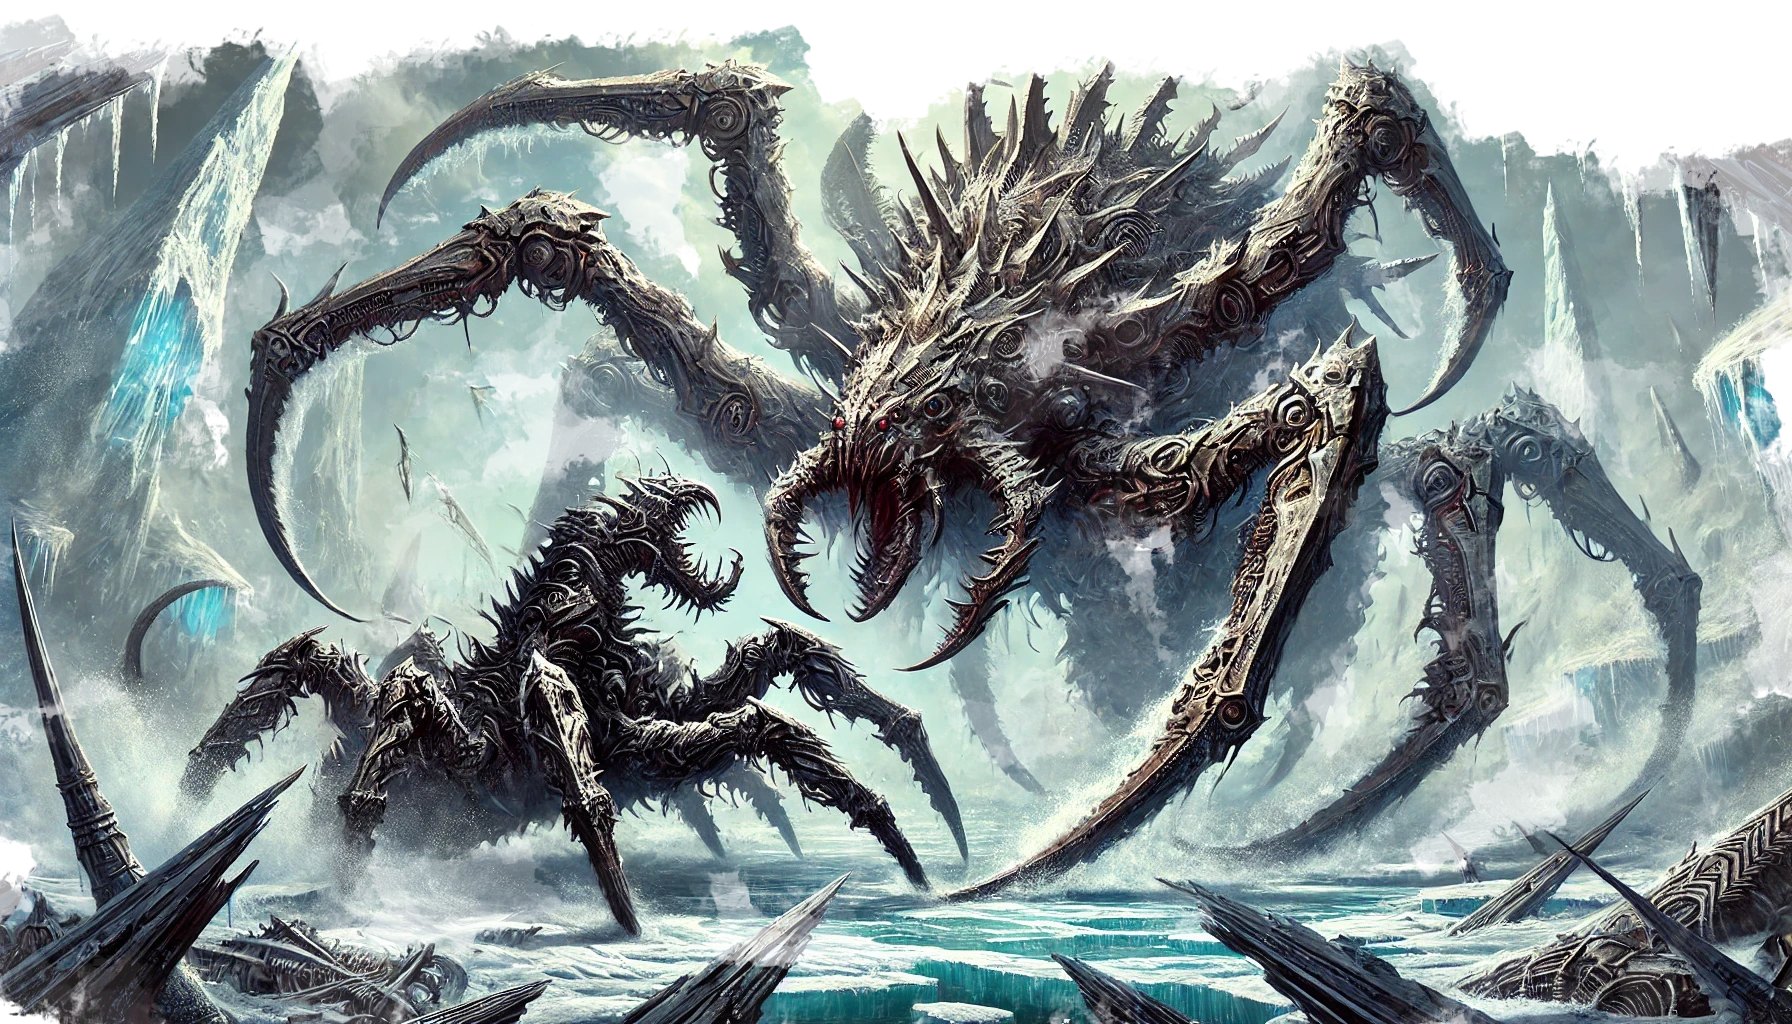
\includegraphics[width=\paperwidth]{images/Spider_Octopus}%
      	\end{minipage}%
	};%
\end{tikzpicture}%
\vspace*{-2.7\fontdimen6\font}\hfill\\
\begin{DndMonster}[width=0.5\textwidth]{Giant Octopus}
	\DndMonsterType{Large Beast, unaligned}
	
	\DndMonsterBasics[
		armor-class	= {\intcalcAdd{13}{\intcalcAdd{1}{\calculateModifier{\WisdomScoreValue}}} (Natural Armor)},
		hit-points	= {\MaxHitPointsValue\ + \intcalcMul{3}{\MultiClassLevelValue} temp HP},
		speed		= {10 ft., swim 60 ft.},
		initiative	= +1,
	]
	
	\renewcommand{\AbilityScoreSpacer}{~}
	
	\DndMonsterAbilityScores[
		str = 17,
		dex = 13,
		con = 13,
		int = 10,
		wis = 18,
		cha = 18,
	]
	
	\DndMonsterDetails[
		%saving-throws			= {},
		skills					= {Perception +7, Stealth +7},
		%damage-vulnerabilities	= {},
		%damage-resistances		= {},
		%damage-immunities		= {},
		%condition-immunities	= {},
		senses					= {Darkvision 60 ft., Passive Perception 17},
		languages				= -,
		challenge				= 1,
		proficiency-bonus		= +3,
	]
	
	\DndMonsterAction{Hold Breath} While out of water, the octopus can hold its breath for 1 hour.
	
	\DndMonsterAction{Underwater Camouflage} The octopus has advantage on Dexterity (Stealth) checks made while underwater.
	
	\DndMonsterAction{Water Breathing} The octopus can breath only underwater.
	
	\DndMonsterSection{Actions}
	\DndMonsterAttack[
		name			= Tentacles,
		distance		= melee,
		%type			= weapon,
		mod				= +7,
		reach			= 15,
		%range			= 20/60,
		targets			= one target,
		dmg				= \DndDice{2d6 + 4},
		dmg-type		= bludgeoning,
		%plus-dmg		= ,
		%plus-dmg-type	= ,
		%or-dmg			= ,
		%or-dmg-when	= ,
		extra			= {. If the target is a creature, it is grappled (escape DC 17). Until this grapple ends, the target is restrained, and the octopus can't use its tentacles on another target},
	]
	\DndMonsterAttack[
		name			= Armblade,
		distance		= melee,
		%type			= weapon,
		mod				= +7,
		reach			= 5,
		%range			= 20/60,
		targets			= one target,
		dmg				= \DndDice{1d8 + 4},
		dmg-type		= slashing,
		%plus-dmg		= ,
		%plus-dmg-type	= ,
		%or-dmg			= ,
		%or-dmg-when	= ,
		%extra			= {},
	]
	
	\DndMonsterAction{Ink Cloud (Recharges after a Short or Long Rest)}
	A 20-foot-radius cloud of ink extends all around the octopus if it is underwater. The area is heavily obscured for 1 minute, although a significant current can disperse the ink. After releasing the ink, the octopus can use the Dash Action as a Bonus Action.
\end{DndMonster}
\vfill\eject
\section*{Brown Bear}
\begin{DndMonster}[width=0.5\textwidth]{Brown Bear}
	\DndMonsterType{Large Beast, unaligned}
	
	\DndMonsterBasics[
		armor-class	= {\intcalcAdd{13}{\intcalcAdd{1}{\calculateModifier{\WisdomScoreValue}}} (Natural Armor)},
		hit-points	= {\MaxHitPointsValue\ + \intcalcMul{3}{\MultiClassLevelValue} temp HP},
		speed		= {40 ft., climb 30 ft.},
		initiative	= +1,
	]
	
	\renewcommand{\AbilityScoreSpacer}{~}
	
	\DndMonsterAbilityScores[
		str = 19,
		dex = 12,
		con = 16,
		int = 10,
		wis = 18,
		cha = 18,
	]
	
	\DndMonsterDetails[
		%saving-throws			= {},
		skills					= {Perception +7},
		%damage-vulnerabilities	= {},
		%damage-resistances		= {},
		%damage-immunities		= {},
		%condition-immunities	= {},
		senses					= {Passive Perception 17},
		languages				= -,
		challenge				= 1,
		proficiency-bonus		= +3,
	]
	
	\DndMonsterAction{Keen Smell} The bear has advantage on Wisdom (Perception) checks that rely on smell.
	
	\DndMonsterSection{Actions}
	
	\DndMonsterAction{Multiattack}
	The bear makes two attacks: one with its bite and one with its claws.
	
	\DndMonsterAttack[
		name			= Bite,
		distance		= melee,
		%type			= weapon,
		mod				= +8,
		reach			= 5,
		%range			= 20/60,
		targets			= one target,
		dmg				= \DndDice{1d8 + 5},
		dmg-type		= piercing,
		%plus-dmg		= ,
		%plus-dmg-type	= ,
		%or-dmg			= ,
		%or-dmg-when	= ,
		%extra			= {},
	]
	\DndMonsterAttack[
		name			= Claws,
		distance		= melee,
		%type			= weapon,
		mod				= +8,
		reach			= 5,
		%range			= 20/60,
		targets			= one target,
		dmg				= \DndDice{2d6 + 5},
		dmg-type		= slashing,
		%plus-dmg		= ,
		%plus-dmg-type	= ,
		%or-dmg			= ,
		%or-dmg-when	= ,
		%extra			= {},
	]
	\DndMonsterAttack[
		name			= Armblade,
		distance		= melee,
		%type			= weapon,
		mod				= +8,
		reach			= 5,
		%range			= 20/60,
		targets			= one target,
		dmg				= \DndDice{1d8 + 5},
		dmg-type		= slashing,
		%plus-dmg		= ,
		%plus-dmg-type	= ,
		%or-dmg			= ,
		%or-dmg-when	= ,
		%extra			= {},
	]
\end{DndMonster}

\part*{Magic Items}

\subsection*{Ventilating Lungs}
\textit{Wondrous Item, rare (requires attunement)}\\
These metallic nodules were created in response to the poisonous gases used on the battlefields of the Last War. When you attune to these lungs, they replace the lungs in your chest, which disappear. The lungs allow you to breathe normally, even in an antimagic field, and their breathing function can't be suppressed by magic.

Outside an antimagic field or any other effect that suppresses magic, these lungs allow you to breathe normally in any environment (including a vacuum), and you have advantage on saving throws against harmful gases such as those created by a Cloudkill spell, a Stinking Cloud spell, inhaled poisons, and gaseous breath weapons .

As an action, you can use these lungs to exhale a gust of wind, as if you had cast the Gust of Wind spell (spell save DC 15) with no components. This property of the lungs can't be used again until the next dawn.

If your attunement to the lungs ends, your original lungs reappear.

\DndSpellHeader
  {Gust of Wind}
  {2nd-Level Evocation}
  {Action}
  {Self (60-footline)}
  {V, S}
  {Concentration, up to 1 Minute}

A line of strong wind 60 feet long and 10 feet wide blasts from you in a direction you choose for the spell's duration. Each creature that starts its turn in the line must succeed on a DC 15 Strength saving throw or be pushed 15 feet away from you in a direction following the line.

Any creature in the line must spend 2 feet of movement for every 1 foot it moves when moving closer to you.

The gust disperses gas or vapor, and it extinguishes candles, torches, and similar unprotected flames in the area. It causes protected flames, such as those of lanterns, to dance wildly and has a 50 percent chance to extinguish them.

As a bonus action on each of your turns before the spell ends, you can change the direction in which the line blasts from you.
\vfill\eject
\subsection*{Insignia of Claws}
\textit{Wondrous Item, uncommon}\\
The jewels in this insignia of the Cult of the Dragon flare with purple light when you enter combat, empowering your natural fists or natural weapons.

While wearing the insignia, you gain a +1 bonus to the attack rolls and the damage rolls you make with unarmed strikes and natural weapons. Such attacks are considered to be magical.

\subsection*{Armblade +1}
\textit{Weapon, uncommon (requires attunement by a warforged)}\\
An armblade is a magic weapon that attaches to your arm, becoming inseparable from you as long as you're attuned to it. To attune to this item, you must hold it against your forearm for the entire attunement period.

As a bonus action, you can retract the armblade into your forearm or extend it from there. While it is extended, you can use the weapon as if you were holding it, and you can't use that hand for other purposes.

\end{document}